\documentclass[xcolor={table, dvipsnames}]{beamer}
\usepackage[utf8]{inputenc,vietnam}

\usepackage{utopia} %font utopia imported
\usetheme{Madrid}
\usecolortheme{default}

% Code syntax highlighter
% https://latex-beamer.com/tutorials/beamer-code/
% Install required tool https://pygments.org/
% Add to PATH: texmaker > Preference
% e.g. /Users/minhnt/Library/Python/3.8/bin
\usepackage{minted}

\usepackage{hyperref}
\hypersetup{
    colorlinks=true,
    linkcolor=blue,
    filecolor=magenta,      
    urlcolor=cyan,
}

\urlstyle{same}

\newcommand\boldblue[1]{\textcolor{blue}{\textbf{#1}}}

\titlegraphic{
\includegraphics[width=.3\textheight,height=.3\textheight]{qrcode.png}}

%------------------------------------------------
%Information to be included in the title page:
\title{Transaction Management}

\subtitle{Concurrency Control with Transactions and Locking Protocols}

%
%\author{Nguyen The Minh}
%\institute{Electronics and Computer Science Home}
%\date{Computing Conference, Oct 2050}
%

%\logo{
\includegraphics[height=1.5cm]{atom.png}}

%End of title page
%-------------------------------------------------

%------------------------------------------------------------
%The next block of commands puts the table of contents at the 
%beginning of each section and highlights the current section:

\AtBeginSection[]
{
  \begin{frame}
    \frametitle{Nội dung}
    \tableofcontents[currentsection]
  \end{frame}
}
%------------------------------------------------------------

\begin{document}

\frame{\titlepage}

%---------------------------------------------------------
%This block of code is for the table of contents after
%the title page
\begin{frame}
\frametitle{Nội dung}
\tableofcontents
\end{frame}
%---------------------------------------------------------

\section{Xử lý dữ liệu đồng thời và toàn vẹn}

\begin{frame}
\frametitle{Khái niệm Transaction}
Transaction:
\begin{itemize}
\item Logical, atomic unit of work, gồm một hay nhiều SQL statements
\item Tất cả statements đều commited hoặc rolled back - all or nothing
\item Transaction unique identifier - transaction ID
\end{itemize}
Các thao tác với database sẽ được thực hiện thông qua transactions.
\end{frame}

\begin{frame}
\frametitle{Cấu trúc của một transaction}
\begin{block}{Explicit transaction}
BEGIN;\\
Statement 1;\\
Statement 2;\\
...\\
COMMIT or ROLLBACK;\\
\end{block}
Implicit transaction: mặc định cho từng SQL statement
\end{frame}

\begin{frame}
\frametitle{Data concurrency and consistency}
DBMS cần đảm bảo:
\begin{itemize}
\item Nhiều users có thể access dữ liệu cùng một lúc (data concurrency)
\item Mỗi user đều thấy dữ liệu toàn vẹn (data consistency)
\end{itemize}
DBMS sẽ hỗ trợ chạy đồng thời nhiều transactions, hỗ trợ và cung cấp phương thức đảm bảo dữ liệu toàn vẹn.
\end{frame}

\begin{frame}
\frametitle{Bài toán quản lý tài khoản ngân hàng}
Chức năng:
\begin{itemize}
\item Tạo tài khoản - account
\item Thêm hay rút tiền từ account
\item Chuyển tiền từ account này sang account khác
\item Gửi tiết kiệm
\item Cộng tiền tiết kiệm hàng tháng
\end{itemize}
\end{frame}

\begin{frame}
\frametitle{Bài toán quản lý tài khoản ngân hàng}
Các bảng dữ liệu:
\begin{itemize}
\item $account(account\_id, balance)$
\item $saving(saving\_id, acount\_id, amount, period, percent, start\_time)$
\item $transaction(xid, type, content, status, xtime)$
\end{itemize}
Có những trường hợp xung đột dữ liệu nào? (inconsistency)
\end{frame}

\begin{frame}
\frametitle{Multiversion Concorrency Model}

\end{frame}

% Locking Mechanisms %
\section{Cơ chế Locking}

\begin{frame}
\frametitle{Tổng quan cơ chế Locking}
\textbf{Lock} là cơ chế bảo vệ dữ liệu khi có nhiều truy cập đồng thời.\\
Cùng với transactions, locking hỗ trỡ data concurrency và consistency.\\
\pause
Có hai loại lock:
\begin{itemize}
\item Exclusive locks và share locks.
\item Chỉ 1 exclusive lock với một resource (a row, a table), share locks có thể nhiều.
\item Lock ảnh hưởng đến readers và writers (query và modifying a resource).
\end{itemize}
\end{frame}

\begin{frame}
\frametitle{Readers và Writers}
Các rules dành cho readers và writers:
\begin{itemize}
\item Một row bị locked chỉ khi thay đổi bởi writer. Một statement update 1 row, transaction acquire 1 row lock.
\item Một writer sẽ block concurrent writers của cùng một row. Một transaction đang update 1 row thì row lock sẽ ngăn transaction khác sửa row đó.
\item A reader never blocks a writer. Reader của một row không lock nó, writer có thể sửa row này. Ngoại trừ $SELECT ... FOR UPDATE$ statement.
\item A writer never blocks a reader. Khi a row đang được thay đổi bởi một writer, DBMS sẽ sử dụng data version cũ cung cấp cho reader.
\end{itemize}
\end{frame}

\begin{frame}
\frametitle{Sử dụng Locks}
DBMS hỗ trợ data concurrency, consistency thông qua việc sử dụng transactions và cơ chế locking.\\
Locking thường sẽ xảy ra tự động mà không cần user tác động gì cả.\\
DBMS sẽ tự động lấy locks khi thực thi SQL statements, trước khi thay đổi dữ liệu thì cần lock lại.\\
DBMS cũng cho phép user sử dụng locking khi cần thiết.\\
\end{frame}

\begin{frame}
\frametitle{Lock Modes}
\begin{block}{Exclusive lock mode}
Bảo vệ dữ liệu tránh shared. Transaction lấy một exclusive lock khi nó thay đổi dữ liệu và chỉ transaction có lock được thay đổi dữ liệu cho đến khi nó release lock. 
\end{block}
\pause
\begin{block}{Share lock mode}
Cho phép share dữ liệu. Nhiều transactions cùng đọc dữ liệu, mỗi thằng sẽ giữ một share lock để tránh transaction writer truy cập.
\end{block}
\end{frame}

\section{Explicit Locking}

\begin{frame}
\frametitle{Lock dữ liệu manual}
Mặc dù DBMS sẽ tự động lock dữ liệu khi cần thiết, nhưng chúng ta có thể manual lock dữ liệu khi DBMS không đáp ứng được mong muốn.\\
Ví dụ, DBMS sẽ lấy share lock cho các câu lệnh SELECT. Nhưng nếu bạn muốn các transaction khác không được SELECT hay UPDATE dữ liệu dùng chung, chúng ta có thể chỉ định exclusive lock bằng SELECT ... FOR UPDATE.
\end{frame}

\begin{frame}
\frametitle{Table-level lock modes}
Transaction có thể lock toàn bộ bảng và hai transaction không thể cùng giữa locks conflict nhau.
\begin{itemize}
\item ACCESS SHARE: Các câu lệnh query sẽ lock bảng ở mode này, conflict với ACCESS EXCLUSIVE.
\item ROW SHARE: SELECT FOR UPDATE, SELECT FOR SHARE dùng mode này, conflict với ACCESS EXCLUSIVE.
\item ROW EXCLUSIVE: UPDATE, DELETE, INSERT dùng mode này, onflict với ACCESS EXCLUSIVE.
\item ACCESS EXCLUSIVE: DROP TABLE, TRUNCATE sử dụng, conflict với ACCESS SHARE, ROW SHARE, ROW EXCLUSIVE
\end{itemize}
https://dev.mysql.com/doc/refman/8.0/en/lock-tables.html\\
https://www.postgresql.org/docs/current/sql-lock.html
\end{frame}

\begin{frame}
\frametitle{Row-level lock modes}
Khác với Table-level lock modes, row-level lock chỉ lock các bảng ghi được đang sử dụng bởi transaction.
\begin{itemize}
\item FOR UPDATE: khi dùng SELECT với mode này các row sẽ bị lock và không thể lock, sửa, hay xóa bởi transaction khác.
\item FOR NO KEY UPDATE: giống FOR UPDATE, nhưng không block câu lệnh  SELECT FOR KEY SHARE.
\item FOR SHARE: giống với FOR NO KEY UPDATE, nhưng nó lấy share lock thay vì exclusive lock cho mỗi row. Shared lock sẽ block transaction khác thực hiện UPDATE, DELETE, SELECT FOR UPDATE or SELECT FOR NO KEY UPDATE với các rows, nhưng không block SELECT FOR SHARE or SELECT FOR KEY SHARE.
\item FOR KEY SHARE: giống FOR SHARE, nhưng chỉ block SELECT FOR UPDATE, không block SELECT FOR NO KEY UPDATE.
\end{itemize}
\end{frame}
\begin{frame}
\frametitle{Conflict giữa row-level lock modes}
%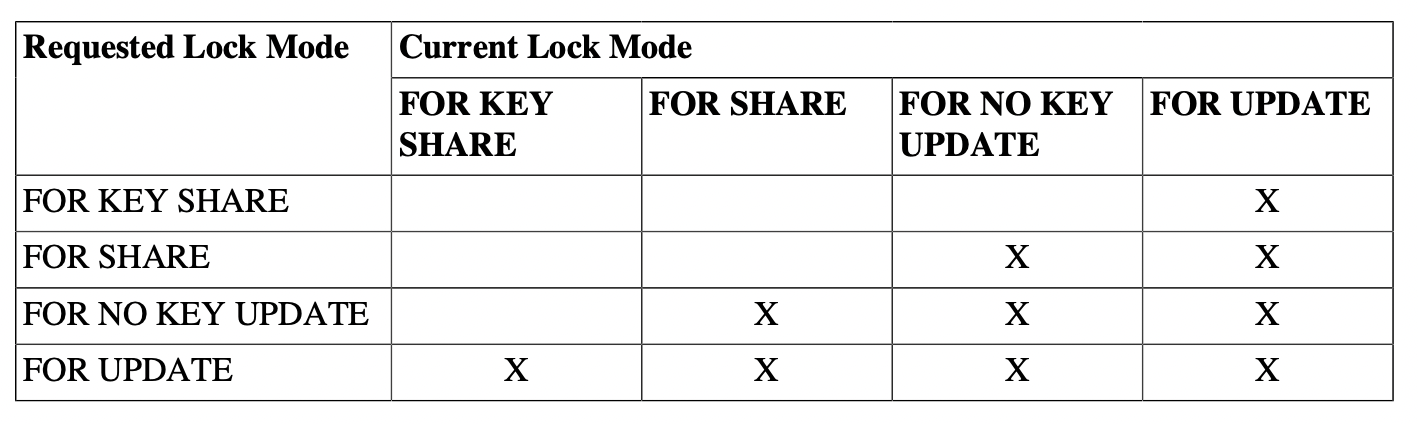
\includegraphics[width=\textheight,height=\textheight]{row-level-lock.png}
https://www.postgresql.org/docs/current/explicit-locking.html
\end{frame}
\end{document}